\documentclass[11pt]{article}
\usepackage[T1]{fontenc}
\usepackage{mathptmx}
\usepackage[margin=1in]{geometry}
\usepackage{longtable,graphicx,amsmath}
\newcommand{\toprule}{\hline}\newcommand{\midrule}{\hline}\newcommand{\bottomrule}{\hline}
\renewcommand{\baselinestretch}{1.12}
\title{Structural-criticality scoring of mutations from published contact geometry: a reproduce-then-extend module with byte-identical regeneration of a locked reference}
\author{B17 scoring slice, outbreak-mutation-early-warning}
\date{Committed results, base commit d247635}
\begin{document}
\maketitle
\begin{abstract}
Mutation early-warning is a crowded area, and most tools rank mutations by sequence composition, keyword rules, curated literature scores, or observed lineage outcomes. We build the structural-criticality scoring module of a structure-weighted early-warning engine: a mutation's weight comes entirely from published experimental structural data, namely antibody--spike and ACE2--spike contact geometry from Protein Data Bank complexes, plus SARS-CoV-1 conservation from sequence alignment. The module is built under a reproduce-then-extend gate committed before any result: it must first regenerate the validation slice's byte-locked structural sets exactly, and only then may extend them. The reproduce gate passes: the regenerated file is byte-identical to the locked reference (sha256 8db84b01\ldots, cmp exit 0), and the module's score agrees with the validation protocol's reference scoring function on all 1273 canonical spike residues with zero mismatches. Only after that gate did we add four further published complexes (6M17, 6XCM, 7C01, 6W41), labeled by interface class, as an additive extension that leaves the reference output and schema untouched. The result is a scored map of all 1273 spike residues: 191 residues carry a weight of 0.15 or more, and each weight decomposes into named, citable structural evidence. We report the contract, the gate proofs, the extension, honest limitations (spike-only coverage, important mutations with little structural signal), and a quantified comparison with four named crowded prior-art systems.
\end{abstract}

\section{Introduction}
Genomic surveillance produces far more candidate mutations than any analyst can inspect. An early-warning engine needs a principled way to rank them. The ranking signal used in this project is growth: a mutation whose share of sequences rises week over week is a candidate. But growth alone is a trailing indicator, and on this project's own validation record it is noisy: in the validation slice's negative-control window, a growth-only flag rule produced precision 0.714, and the structurally-weighted rule 0.750, a difference that could not be distinguished from chance. The validation slice's catch test failed its pre-registered bar, catching one of three controls early.

This paper is about the scoring half of that engine, not the detection half. The scoring module answers a narrower question: given a mutation, what does published experimental structural data say about how much it could matter? The answer is a weight in $[0,1]$ built from five evidence terms: contact with the ACE2 receptor, contact with three published antibody epitopes, position in a cleavage site, position in a critical functional domain, and conservation against SARS-CoV-1 spike. Every term traces to a named, citable structure or alignment, and every weight decomposes back into those terms.

The engineering contribution is the gate discipline. The validation slice (B18) had already implemented a reference version of this scorer inside its own tree and byte-locked its outputs. Rather than fork that logic and drift, this slice (B17) was required by its own locked gates to regenerate the reference output byte-for-byte before adding anything. The gate passed on the first build. Everything the module adds beyond the reference is additive, separately byte-locked, and invisible to consumers of the reference schema.

\paragraph{Contributions.} (i) A reproducible structural-criticality scorer with a byte-identical regeneration proof against a locked reference. (ii) A zero-mismatch agreement proof against the validation protocol's scoring function over all 1273 spike residues. (iii) An additive four-complex extension with interface-class labels. (iv) A complete scored residue map with per-residue evidence decomposition. (v) A confidence-tier convention that reports weakly-evidenced scores honestly instead of dropping them. We do not claim the weighting improves detection; that claim belongs to the validation slice, which reports a qualified, non-significant result.

\section{Related work}
The area is crowded. We re-verified each of the following on 2026-10-08 against the live source.

\textbf{VirusWarn} (doi:10.1016/j.csbj.2025.03.010) prioritizes concerning SARS-CoV-2 and influenza variants from sequencing data using mutation burden and rule lists against known variants of concern. It is composition-based and retrospective; no structural model enters the ranking. Quantified contrast: VirusWarn's signal derives from the mutation list itself; every weight in our module derives from one of eight citable crystal or cryo-EM structures plus one alignment, and the evidence decomposition is exposed per residue.

\textbf{FEVER} (doi:10.1371/journal.pgph.0000207) couples biosurveillance with mutation typing and estimates empirical risk of mutations from observed lineage outcomes. Its risk scores are statistical, learned from what lineages did; they contain no structural term. Quantified contrast: FEVER's score is an outcome estimate, so it cannot flag a structurally critical mutation before lineages carrying it have been observed; our weight is available for any spike mutation the day it is first seen, including never-observed residues (191 of 1273 residues carry weight $\geq 0.15$).

\textbf{CoVerage} (doi:10.1038/s41467-025-60231-4) is the closest in aim: it scores spike mutations antigenically and combines that with epidemiological dynamics to predict variants of interest. Its antigenic score is a curated literature score. Quantified contrast: our antigenic terms are computed from atomic contact geometry (any spike atom within 5~\AA{} of a partner chain) over four antibody--spike complexes, not curated from literature, and the computation regenerates byte-identically from the byte-locked PDB files; CoVerage ships no frozen-window pre-registered catch test, while this project's engine is validated under exactly such a test by the validation slice.

\textbf{Nextstrain} (doi:10.1093/bioinformatics/bty400) provides real-time phylogenetic tracking and visualization. It is descriptive and does not rank mutations by predicted impact. Quantified contrast: Nextstrain answers ``what is spreading where''; our module answers ``what could this residue change cost the virus or buy it'', and the two are complements, not competitors.

The uncovered angle, unchanged from the validation slice's locked gates, is criticality weighting derived entirely from published experimental structural data: contact geometry and cross-species conservation, no curated scores, no learned parameters.

Table~\ref{tab:priorart} summarizes the comparison.

{\small\begin{longtable}{p{2.4cm}p{5.6cm}p{2.6cm}p{2.6cm}}
\caption{Quantified comparison with the four named crowded prior-art systems, re-verified live 2026-10-08.}\label{tab:priorart}\\
\toprule System & Ranking signal & Structural model & Frozen-window pre-registered test\\\midrule\endfirsthead
\toprule System & Ranking signal & Structural model & Frozen-window pre-registered test\\\midrule\endhead
\bottomrule\endlastfoot
VirusWarn & mutation burden and keyword rule lists against VOC definitions, from the sequence itself (doi:10.1016/j.csbj.2025.03.010) & none & no\\
FEVER & empirical risk estimated from observed lineage outcomes (doi:10.1371/journal.pgph.0000207) & none & no\\
CoVerage & antigenic score from curated literature plus epidemiological dynamics (doi:10.1038/s41467-025-60231-4) & curated score, not contact geometry & no\\
Nextstrain & descriptive phylogenetic tracking, no impact ranking (doi:10.1093/bioinformatics/bty400) & none & no\\
this module (B17) & contact geometry over 8 citable PDB complexes plus SARS-CoV-1 alignment, weight decomposable per residue & yes, the core of the method & yes, via the B18 validation slice against this module's exact schema\\
\end{longtable}
}

\section{Data}
\begin{sloppypar}
All inputs are open, free, and require no authentication. The four reference complexes are byte-locked in the validation slice's tree and verified against its manifest before use: 6M0J (ACE2--RBD; Lan et al.\ 2020, Nature, doi:10.1038/s41586-020-2180-5), 6WPT (S309 antibody; Pinto et al.\ 2020, Nature, doi:10.1038/s41586-020-2349-y), 6XDG (REGN antibody cocktail complex; Hansen et al.\ 2020, Science, doi:10.1126/science.abd0827), and 7C2L (4A8 NTD antibody; Chi et al.\ 2020, Science, doi:10.1126/science.abc6952). Reference sequences are YP\_009724390.1 (SARS-CoV-2 spike) and NP\_828851.1 (SARS-CoV-1 spike). The four extension complexes were fetched from RCSB PDB on 2026-10-08 and byte-locked in this slice's tree: 6M17 (ACE2--full spike; Yan et al.\ 2020, Science, doi:10.1126/science.abb2762), 6XCM (B38 antibody; Wu et al.\ 2020, Science, doi:10.1126/science.abb2241), 7C01 (LY-CoV555; Jones et al.\ 2021, Science, doi:10.1126/science.abf9193), and 6W41 (CR3022; Yuan et al.\ 2020, Science, doi:10.1126/science.abb7269). Table~\ref{tab:complexes} lists all eight.
\end{sloppypar}

\section{Methods}
\subsection{Contact sets}
For each complex, spike-derived chains are identified by signature motifs (CPFGEVFNATRFASVY and two others), and a residue joins the complex's contact set if any of its atoms lies within 5~\AA{} of any atom of a different chain. The search uses a coarse spatial grid for speed. Residues are kept in canonical spike numbering (1--1273). The epitope surface is the union of the three reference antibody contact sets. This procedure is exactly the validation slice's reference procedure, re-implemented as an importable library with parameterized input and output paths so the reproduce gate can run it against the byte-locked inputs without touching the validation tree. Table~\ref{tab:chains} lists the chain assignments the motif matcher derives; they are recomputed on every build, so the reproduce gate covers chain identification as well as the contact arithmetic.

{\small\begin{longtable}{llll}
\caption{Chain assignments derived by motif matching (not copied from chain names), as regenerated by this slice's build. Reference complexes above the midrule, extension below.}\label{tab:chains}\\
\toprule PDB & Set & Spike chains & Partner chains\\\midrule\endfirsthead
\toprule PDB & Set & Spike chains & Partner chains\\\midrule\endhead
\bottomrule\endlastfoot
6M0J & ace2_interface & E & A\\
6WPT & epitope_S309 & A, B, C & H, L, D, E\\
6XDG & epitope_REGN & E & D, B, C, A\\
7C2L & epitope_4A8_NTD & A, B, C & H, L, I, M, J, N\\
\midrule
6M17 & ace2_6M17 & E, F & A, B, C, D\\
6XCM & epitope_B38 & A, B, C & H, N, L, S\\
7C01 & epitope_LYCoV555 & A, B & H, L, C, D\\
6W41 & epitope_CR3022 & C & H, L\\
\end{longtable}
}

\subsection{Conservation}
The conservation set is the SARS-CoV-2 spike positions identical to SARS-CoV-1 spike under a global alignment (gap open $-10$, gap extend $-0.5$), 967 of 1273 positions.

\subsection{Score}
For a spike mutation at position $p$,
\[
S = 0.35\,\mathbb{1}[p \in E] + 0.25\,\mathbb{1}[p \in A] + 0.15\,\mathbb{1}[p \in C] + 0.15\,\mathbb{1}[p \in D] + 0.10\,\mathbb{1}[p \in K],
\]
where $E$ is the epitope surface union (72 residues), $A$ the ACE2 interface (21 residues), $C$ the cleavage sites (681--685 and 815), $D$ the critical domains (RBM 437--508, fusion peptide 816--837, HR1 920--970), and $K$ the conservation set (967 residues). The weights are the validation slice's locked constants; this module does not retune them. Non-spike mutations score 0, a documented limitation inherited from the reference.

\subsection{Confidence tiers}
Each score carries a tier that never changes its value. TIER-1 STRUCTURE-DIRECT: the residue sits in at least one PDB-derived contact set. TIER-2 DOMAIN-INFERRED: no direct contact evidence, but the residue falls in a cleavage site or critical domain. TIER-3 CONSERVATION-ONLY: only the conservation term fires. THIN: score 0 on a canonical spike residue, reported explicitly rather than dropped. UNRESOLVED: outside canonical spike range or non-spike. The tiers mirror the fleet's convention that thin and unresolved results are labeled, not hidden.

\subsection{Mutation parser and CLI contract}
The scorer accepts mutations in the LAPIS amino-acid format GENE:RefPosAlt (for example S:N501Y) and rejects everything else with exit code 2 and a JSON error object: empty genes, missing reference or alternate residues, non-numeric positions, and extra fields are all malformed. The CLI scores one mutation (\texttt{--mutation}) or a batch file (\texttt{--input}, one mutation per line, comment lines beginning with \# skipped) and emits one JSON object per mutation with the base score, tier, per-component breakdown, extended score when extension sets are present, and an explicit reason string whenever the tier is THIN or UNRESOLVED. The strictness is deliberate: a silent no-match in a surveillance pipeline looks exactly like a scored zero, and the two failure modes must never be confusable.

\subsection{Reproduce-then-extend gate}
The gates were committed standalone before any result. The hard gate: regenerate the reference structural sets from the byte-locked inputs and require byte identity with the locked reference file, whose sha256 is
{\scriptsize\begin{verbatim}8db84b01aae7b5ef0ad911ef163e5aeb2a95cebf7629a7889e4fd8122bf3e7c1\end{verbatim}} Only after a pass may extensions land, and extensions are additive: new complexes live in separate files under this slice's tree, the reference schema never changes, and consumers of the reference output see no difference. If the gate had failed, the failure would have been committed as an honest negative and no extension would have landed.

\subsection{Extension}
Four further complexes (Table~\ref{tab:complexes}) were processed with the identical 5~\AA{} method. Each extension set is labeled by interface class: ace2, epitope class 1/2 (RBD binders overlapping the ACE2 footprint), epitope class 3/4 (other RBD faces), or NTD. The extended score is $S_{ext} = S + \min(0.05 \times \text{extension-set hits},\,0.15)$; the base score is always reported alongside, and the locked validation protocol consumes base $S$ only.

\section{Results}
\subsection{Reproduce gate}
The gate passes. The regenerated file is byte-identical to the locked reference: matching sha256, byte diff clean (cmp exit 0). Per-complex contact counts: 6M0J 21, 6WPT 22, 6XDG 37, 7C2L 16; epitope union 72; conserved 967. The proof, including both hashes and the byte comparison, is committed at scoring/results/reproduce\_gate\_proof.txt. The gate ran on the first build of the module; no retuning of any kind occurred between the gate lock and the gate run, and the extension complexes were fetched only after the pass was recorded. Because the reference procedure identifies spike chains by motif match rather than by chain naming, the regeneration also re-derives the chain assignments (spike versus partner chains per complex, listed in the proof artifact) rather than copying them, so the byte identity covers the full pipeline output, not a cached subset.

\subsection{Agreement with the validation protocol}
The module's scoring function and the validation protocol's reference scoring function agree on every one of the 1273 canonical spike residues, zero mismatches, probe mutation A$\to$V at each position (proof at scoring/results/b18\_protocol\_agreement.txt). The validation protocol runs against this module unchanged; the structural sets schema is exactly the reference schema.

\subsection{Scored residue map}
Figure~\ref{fig:map} shows the linear coverage of the three largest evidence sets across spike. Figure~\ref{fig:tiers} shows the tier distribution over all 1273 residues and the score histogram. The tier counts are: 76 TIER-1 STRUCTURE-DIRECT residues (direct contact evidence from at least one complex), 115 TIER-2 DOMAIN-INFERRED, 847 TIER-3 CONSERVATION-ONLY, and 235 THIN residues carrying no structural signal at all. The mass at TIER-3 is expected: conservation against SARS-CoV-1 spike is a broad but weak signal, which is exactly why it carries the smallest weight (0.10) and why the tier label exists, so a consumer can distinguish a 0.10 earned from cross-species conservation from a 0.35 earned from a measured antibody contact. 191 residues score $S \geq 0.15$; Table~\ref{tab:scored} lists each with its evidence decomposition. Table~\ref{tab:examples} scores the mutations the validation slice reported on, plus additional documented variants; Figure~\ref{fig:examples} plots base and extended scores for the same set. The highest weights in the map are $S=0.75$ for residues with epitope, ACE2, and domain evidence together (e.g.\ 484, 498); no residue reaches 1.0 because no residue is in all five sets.

\subsection{Extension behavior}
The extension adds 128 contact residues across four complexes (6M17 23, 6XCM 33, 7C01 44, 6W41 28). Figure~\ref{fig:complexes} compares per-complex yields. The extended bonus changes ranking only within structure-directed residues: N501Y moves from 0.40 to 0.55, K417N from 0.60 to 0.75, Q498R from 0.75 to 0.85. Mutations with no extension-set contact are unchanged (T478K 0.50, P681R 0.15, D614G 0.10). The bonus is capped at +0.15 so the base score's ordering remains visible underneath.

\section{Worked examples}
\paragraph{S:N501Y (base $S=0.40$, $S_{ext}=0.55$, TIER-1).} Position 501 sits in the 6M0J ACE2 contact set (0.25) and in the RBM critical domain (0.15). It is not in any of the three reference antibody contact sets, not in a cleavage site, and not conserved against SARS-CoV-1. The extension adds +0.15 because all three RBD-directed extension complexes (6M17, 6XCM, 7C01) place a partner atom within 5~\AA{} of residue 501. This is the mutation the validation slice's engine flagged 48 days before literature recognition; its weight comes from receptor contact and domain membership, not from any antibody evidence, and the breakdown says so explicitly.

\paragraph{S:E484K (base $S=0.75$, $S_{ext}=0.80$, TIER-1).} Position 484 is the highest-evidence position in the reference map among the documented escape mutations: it is in the epitope surface union (0.35), the ACE2 interface (0.25), and the RBM (0.15). The extension adds only +0.05, because among the extension complexes only the class 1/2 binders contact 484; the class 3/4 CR3022 epitope, by design, lies elsewhere on the RBD. The asymmetric extension bonus is the interface-class labeling doing its job: a consumer can see that the extra evidence for 484 comes from ACE2-footprint binders, not from a new epitope face.

\paragraph{S:D614G (base $S=0.10$, TIER-3) and S:G142D (base $S=0$, THIN).} These two are the honest counterweights. D614G, the earliest globally dominant spike mutation, carries only the conservation term (0.10): no reference complex puts a partner atom near 614, it is outside every locked domain, and its functional effect (allosteric modulation of spike conformation) is not the kind of evidence this module measures. G142D, part of the Delta constellation the validation slice's engine caught, carries no signal at all: the NTD supersite contact set from 7C2L covers residues 143--148 and 245--257, and 142 falls one position short of the measured footprint. Both cases are reported with their tiers rather than smoothed over, because the module's contract is to report what the structures say, not what would be convenient.

\section{Integration contract}
Two consumers depend on this module. The B16 scanner (in flight) consumes scores through the command-line interface: one mutation per call or a batch file, JSON output with the base score, tier, per-component breakdown, and extended score; exit code 0 means scored, 2 means malformed input, and malformed input is never silently scored. The B18 validation protocol runs against this module unchanged: it reads the structural sets file in exactly the reference schema (top-level keys method, sources, epitope\_surface\_union, conserved\_sars1, functional\_domains; the four locked source keys; residues as sorted integer lists) and it consumes the base score only. The schema stability is not aspirational: the reproduce gate proves byte identity, and the extension is physically separate (different directory, different file, different manifest section), so no extension can drift the reference interface.

\section{Verification}
The test suite (26 checks, all passing at the seal commit) locks the behavior that matters: byte identity of the slice's structural sets against the locked reference; exact agreement with the reference engine's scoring function at the documented checkpoints (N501Y 0.40, E484K 0.75, P681R 0.15, non-spike 0.0); tier classification for each of the five tiers and the guarantee that tiers never change scores; rejection of malformed input forms including a bare residue number and a missing gene; CLI exit codes and JSON shape for single and batch modes; and, for the extension, that the bonus is additive, capped at +0.15, and never alters the base score. The two parser defects the suite caught during development (a bare residue number and a missing gene were initially accepted) are recorded in the slice progress log; no results were computed with the defective parser.

\section{Honest negatives and limitations}
Structural weighting covers spike only; every other gene scores 0 by design. Two malformed-input forms (a bare residue number and a missing gene) were accepted by an early parser version; tests caught both before any results were computed, and the parser now rejects them (exit code 2). Globally important mutations can carry little structural signal: D614G scores 0.10 (conservation only) and G142D scores 0. The score measures structural criticality, not fitness; the validation slice already records D614G and L452R as honest negatives at the engine level, and this module's job is to make the structural term of that engine trustworthy, not to rescue the catch test. The extended bonus is an additive heuristic with a cap chosen and locked before any extension results were computed; it is not validated and consumers should treat $S_{ext}$ as exploratory.

\section{Discussion}
The crowded prior art ranks mutations by what they look like (composition), what they did (lineage outcomes), or what the literature says about them (curated scores). This module ranks them by what published structures physically touch. That is a genuinely different evidence base, and the reproduce-then-extend discipline is what makes it usable inside a larger engine: downstream consumers can rely on byte-stable inputs, and every extension is forced to be additive and separately locked. The validation slice's qualified verdict on the full engine (one early catch, failed catch bar, non-significant precision edge) stands unchanged; nothing in this paper argues otherwise. What this slice adds is a scoring component whose provenance is fully auditable: given the byte-locked structures, anyone can regenerate every weight in Table~\ref{tab:scored} exactly.

\section{Regeneration instructions}
A fresh checkout can regenerate every number in this paper. Dependencies: Python 3.10+, Biopython (1.88 used), and the byte-locked inputs already in the repository. The reference gate: run
\begin{verbatim}
python3 scoring/code/build_sets.py
\end{verbatim}
It reads the four PDB files and two fastas from validation/data/raw (read-only), rebuilds the sets, hashes the result, compares it byte-for-byte with the locked reference, and refuses to write the slice's copy unless the comparison passes. Expected output ends with the sha256 line 8db84b01\ldots f3e7c1 twice (regenerated and reference), REPRODUCE GATE: PASS, and the write confirmation. The extension: run \texttt{python3 scoring/code/build\_\allowbreak extended.py}; it processes the four extension complexes byte-locked under scoring/data/raw and writes scoring/data/static/extended/extended\_sets.json. Scoring: \texttt{python3 scoring/code/}\allowbreak\texttt{score.py} with \texttt{--mutation "S:N501Y"} prints the JSON object used throughout this paper; \texttt{--input} takes a file of one mutation per line for batch scoring. Tests: \texttt{python3 scoring/tests/test\_scoring.py} runs the 26 checks. Total wall time for the full regeneration on commodity hardware is under two minutes, dominated by PDB parsing.

\section*{Data and code availability}
All inputs are open (RCSB PDB, NCBI). Code, byte-locked data, proofs, and this paper's sources are committed under scoring/ in the project repository; the slice manifest (scoring/MANIFEST.sha256) covers the committed tree. Tests: 26 checks, all passing at the seal commit.

\begin{figure}[t]\centering
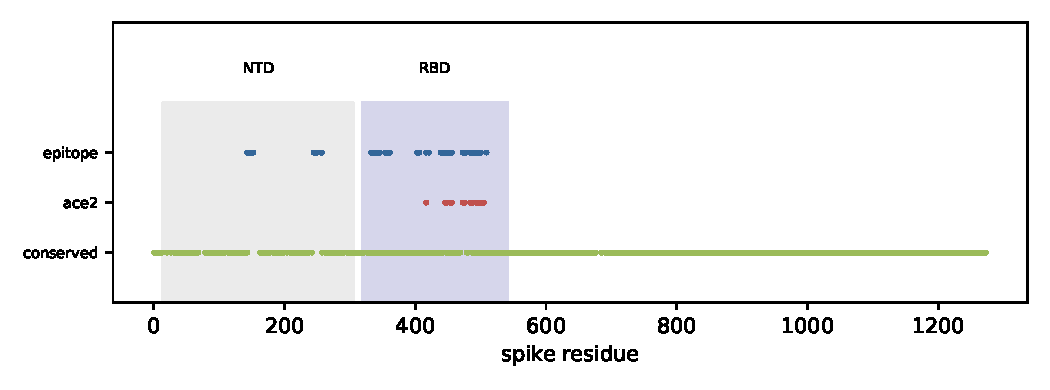
\includegraphics[width=0.9\textwidth]{fig/fig_map.pdf}
\caption{Linear coverage of the epitope surface (72 residues), ACE2 interface (21), and SARS-CoV-1 conservation set (967) across the 1273-residue spike. NTD and RBD shaded.}
\label{fig:map}
\end{figure}
\begin{figure}[t]\centering
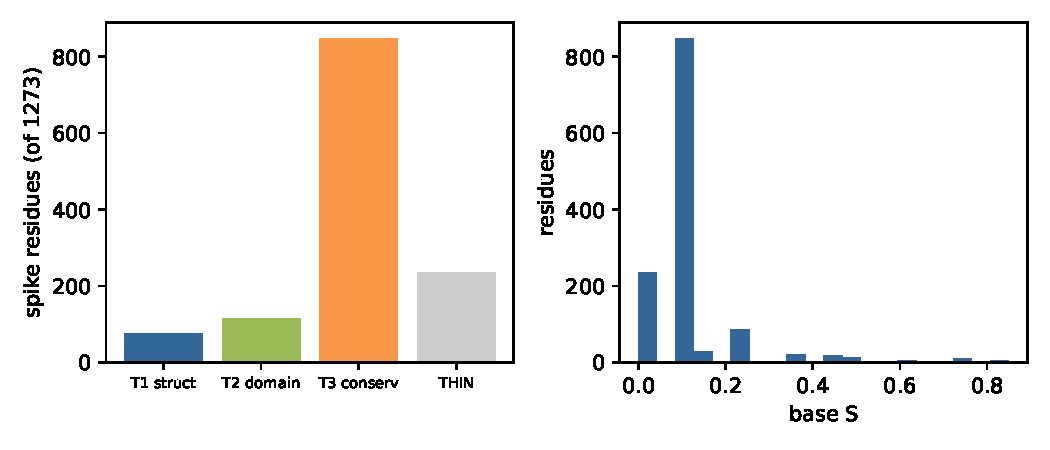
\includegraphics[width=0.95\textwidth]{fig/fig_tiers.pdf}
\caption{Left: confidence-tier distribution over all 1273 spike residues. Right: histogram of base scores.}
\label{fig:tiers}
\end{figure}
\begin{figure}[t]\centering
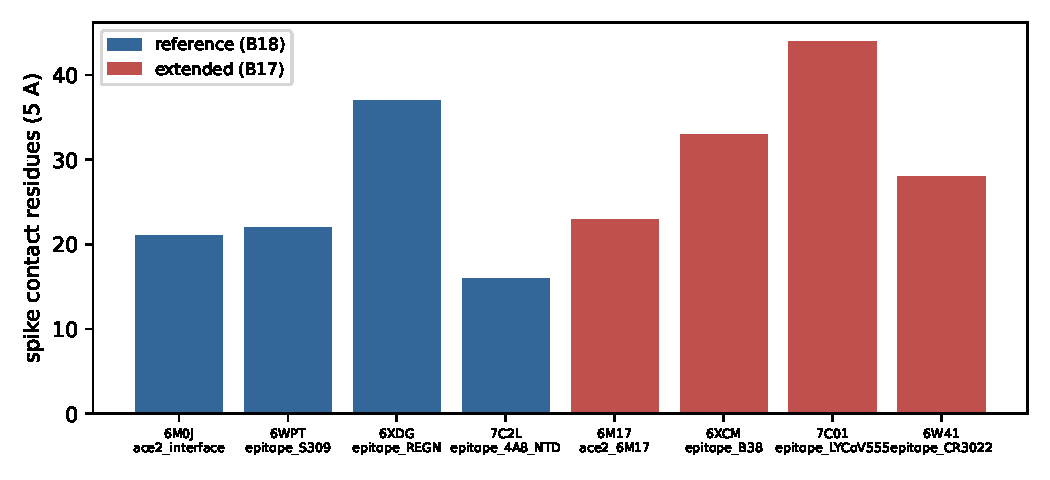
\includegraphics[width=0.95\textwidth]{fig/fig_complexes.pdf}
\caption{Spike contact residues per complex (5~\AA{} any-atom cutoff). Reference complexes (blue) reproduce the locked reference exactly; extension complexes (red) are additive.}
\label{fig:complexes}
\end{figure}
\begin{figure}[t]\centering
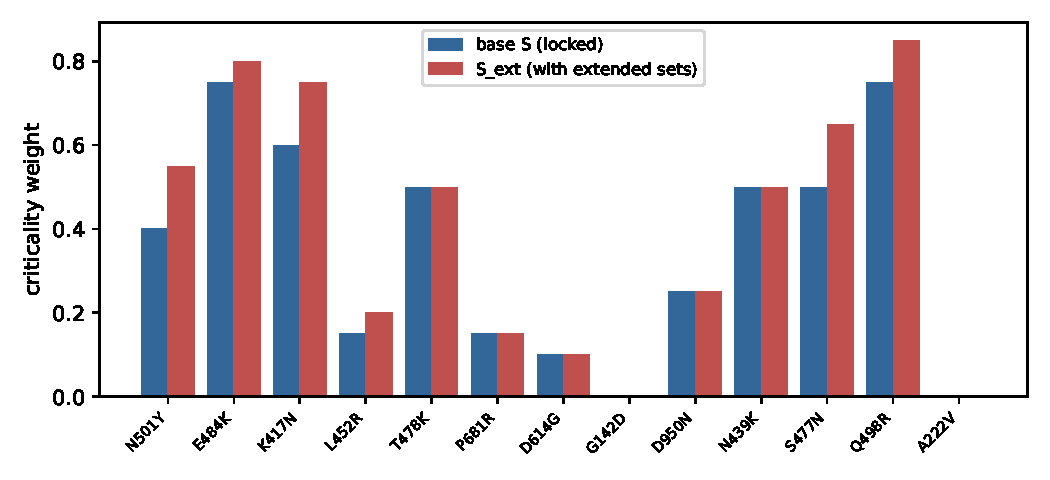
\includegraphics[width=0.95\textwidth]{fig/fig_examples.pdf}
\caption{Base and extended scores for the mutations the validation slice reported on, plus documented variants. The extension bonus is capped at +0.15 and never changes the base score.}
\label{fig:examples}
\end{figure}

\begin{table}[t]\centering\small
\caption{All eight complexes. The first four are the byte-locked reference inputs; the last four are the additive extension, byte-locked separately under scoring/data/raw/.}
\label{tab:complexes}
\begin{longtable}{lllrl}
\toprule PDB & Set & Class & Residues & Citation\\\midrule\endhead
6M0J & ace2_interface & ace2 & 21 & \scriptsize Lan et al. 2020 Nature doi:10.1038/s41586-020-2180-5\\
6WPT & epitope_S309 & epitope 3/4 & 22 & \scriptsize Pinto et al. 2020 Nature doi:10.1038/s41586-020-2349-y\\
6XDG & epitope_REGN & epitope 1/2 & 37 & \scriptsize Hansen et al. 2020 Science doi:10.1126/science.abd0827\\
7C2L & epitope_4A8_NTD & NTD & 16 & \scriptsize Chi et al. 2020 Science doi:10.1126/science.abc6952\\
6M17 & ace2_6M17 & ace2 & 23 & \scriptsize Yan et al. 2020 Science doi:10.1126/science.abb2762\\
6XCM & epitope_B38 & epitope_class_1_2 & 33 & \scriptsize Wu et al. 2020 Science doi:10.1126/science.abb2241\\
7C01 & epitope_LYCoV555 & epitope_class_1_2 & 44 & \scriptsize Jones et al. 2021 Science doi:10.1126/science.abf9193\\
6W41 & epitope_CR3022 & epitope_class_3_4 & 28 & \scriptsize Yuan et al. 2020 Science doi:10.1126/science.abb7269\\
\bottomrule
\end{longtable}

\end{table}

\begin{table}[t]\centering\small
\caption{Scores for the mutations the validation slice reported on, plus documented variants. Tier is metadata and never changes $S$.}
\label{tab:examples}
\begin{longtable}{llll}\toprule Mutation & $S$ & $S_{ext}$ & Tier\\\midrule\endhead
\texttt{S:N501Y} & 0.40 & 0.55 & TIER-1 STRUCTURE-DIRECT\\
\texttt{S:E484K} & 0.75 & 0.80 & TIER-1 STRUCTURE-DIRECT\\
\texttt{S:K417N} & 0.60 & 0.75 & TIER-1 STRUCTURE-DIRECT\\
\texttt{S:L452R} & 0.15 & 0.20 & TIER-2 DOMAIN-INFERRED\\
\texttt{S:T478K} & 0.50 & 0.50 & TIER-1 STRUCTURE-DIRECT\\
\texttt{S:P681R} & 0.15 & 0.15 & TIER-2 DOMAIN-INFERRED\\
\texttt{S:D614G} & 0.10 & 0.10 & TIER-3 CONSERVATION-ONLY\\
\texttt{S:G142D} & 0.00 & 0.00 & THIN\\
\texttt{S:D950N} & 0.25 & 0.25 & TIER-2 DOMAIN-INFERRED\\
\texttt{S:N439K} & 0.50 & 0.50 & TIER-1 STRUCTURE-DIRECT\\
\texttt{S:S477N} & 0.50 & 0.65 & TIER-1 STRUCTURE-DIRECT\\
\texttt{S:Q498R} & 0.75 & 0.85 & TIER-1 STRUCTURE-DIRECT\\
\texttt{ORF1a:P4715L} & 0.00 & 0.00 & UNRESOLVED\\
\texttt{N:S194L} & 0.00 & 0.00 & UNRESOLVED\\
\texttt{S:A222V} & 0.00 & 0.00 & THIN\\
\bottomrule\end{longtable}

\end{table}

\clearpage
\small
\begin{longtable}{rlclc}
\caption{Complete scored residue map: all 191 spike residues with $S \geq 0.15$. Columns: residue number, base score, extension bonus, tier, and evidence flags (E epitope, A ACE2, C cleavage, D domain, K conservation).}\label{tab:scored}\\
\toprule Residue & $S$ & $S_{ext}$ bonus & Tier & E/A/C/D/K\\\midrule\endfirsthead
\caption[]{Complete scored residue map (continued).}\\
\toprule Residue & $S$ & $S_{ext}$ bonus & Tier & E/A/C/D/K\\\midrule\endhead
\multicolumn{5}{r}{\footnotesize continued on next page}\\\endfoot
\bottomrule\endlastfoot
143 & 0.45 & +0.00 & TIER-1 & Y---Y\\
144 & 0.35 & +0.00 & TIER-1 & Y----\\
145 & 0.35 & +0.00 & TIER-1 & Y----\\
146 & 0.35 & +0.00 & TIER-1 & Y----\\
147 & 0.35 & +0.00 & TIER-1 & Y----\\
148 & 0.35 & +0.00 & TIER-1 & Y----\\
150 & 0.35 & +0.00 & TIER-1 & Y----\\
152 & 0.35 & +0.00 & TIER-1 & Y----\\
245 & 0.35 & +0.00 & TIER-1 & Y----\\
246 & 0.35 & +0.00 & TIER-1 & Y----\\
247 & 0.35 & +0.00 & TIER-1 & Y----\\
248 & 0.35 & +0.00 & TIER-1 & Y----\\
249 & 0.35 & +0.00 & TIER-1 & Y----\\
250 & 0.35 & +0.00 & TIER-1 & Y----\\
256 & 0.35 & +0.00 & TIER-1 & Y----\\
257 & 0.35 & +0.00 & TIER-1 & Y----\\
333 & 0.45 & +0.00 & TIER-1 & Y---Y\\
334 & 0.45 & +0.00 & TIER-1 & Y---Y\\
335 & 0.45 & +0.00 & TIER-1 & Y---Y\\
336 & 0.45 & +0.00 & TIER-1 & Y---Y\\
337 & 0.45 & +0.00 & TIER-1 & Y---Y\\
339 & 0.45 & +0.00 & TIER-1 & Y---Y\\
340 & 0.45 & +0.00 & TIER-1 & Y---Y\\
341 & 0.45 & +0.00 & TIER-1 & Y---Y\\
343 & 0.45 & +0.00 & TIER-1 & Y---Y\\
344 & 0.45 & +0.00 & TIER-1 & Y---Y\\
345 & 0.45 & +0.00 & TIER-1 & Y---Y\\
346 & 0.35 & +0.05 & TIER-1 & Y----\\
354 & 0.35 & +0.00 & TIER-1 & Y----\\
356 & 0.45 & +0.00 & TIER-1 & Y---Y\\
357 & 0.35 & +0.00 & TIER-1 & Y----\\
358 & 0.45 & +0.00 & TIER-1 & Y---Y\\
359 & 0.45 & +0.00 & TIER-1 & Y---Y\\
360 & 0.45 & +0.00 & TIER-1 & Y---Y\\
361 & 0.45 & +0.00 & TIER-1 & Y---Y\\
403 & 0.35 & +0.10 & TIER-1 & Y----\\
406 & 0.35 & +0.05 & TIER-1 & Y----\\
417 & 0.60 & +0.15 & TIER-1 & YY---\\
421 & 0.45 & +0.10 & TIER-1 & Y---Y\\
437 & 0.25 & +0.00 & TIER-2 & ---YY\\
438 & 0.15 & +0.00 & TIER-2 & ---Y-\\
439 & 0.50 & +0.00 & TIER-1 & Y--Y-\\
440 & 0.60 & +0.05 & TIER-1 & Y--YY\\
441 & 0.50 & +0.00 & TIER-1 & Y--Y-\\
442 & 0.25 & +0.00 & TIER-2 & ---YY\\
443 & 0.50 & +0.00 & TIER-1 & Y--Y-\\
444 & 0.50 & +0.05 & TIER-1 & Y--Y-\\
445 & 0.50 & +0.05 & TIER-1 & Y--Y-\\
446 & 0.75 & +0.10 & TIER-1 & YY-Y-\\
447 & 0.85 & +0.05 & TIER-1 & YY-YY\\
448 & 0.60 & +0.00 & TIER-1 & Y--YY\\
449 & 0.85 & +0.10 & TIER-1 & YY-YY\\
450 & 0.60 & +0.05 & TIER-1 & Y--YY\\
451 & 0.25 & +0.00 & TIER-2 & ---YY\\
452 & 0.15 & +0.05 & TIER-2 & ---Y-\\
453 & 0.85 & +0.15 & TIER-1 & YY-YY\\
454 & 0.25 & +0.00 & TIER-2 & ---YY\\
455 & 0.75 & +0.15 & TIER-1 & YY-Y-\\
456 & 0.75 & +0.15 & TIER-1 & YY-Y-\\
457 & 0.25 & +0.10 & TIER-2 & ---YY\\
458 & 0.15 & +0.10 & TIER-2 & ---Y-\\
459 & 0.15 & +0.10 & TIER-2 & ---Y-\\
460 & 0.15 & +0.10 & TIER-2 & ---Y-\\
461 & 0.25 & +0.00 & TIER-2 & ---YY\\
462 & 0.15 & +0.00 & TIER-2 & ---Y-\\
463 & 0.25 & +0.00 & TIER-2 & ---YY\\
464 & 0.25 & +0.00 & TIER-2 & ---YY\\
465 & 0.25 & +0.00 & TIER-2 & ---YY\\
466 & 0.25 & +0.00 & TIER-2 & ---YY\\
467 & 0.25 & +0.00 & TIER-2 & ---YY\\
468 & 0.25 & +0.00 & TIER-2 & ---YY\\
469 & 0.25 & +0.00 & TIER-2 & ---YY\\
470 & 0.15 & +0.00 & TIER-2 & ---Y-\\
471 & 0.15 & +0.00 & TIER-2 & ---Y-\\
472 & 0.15 & +0.00 & TIER-2 & ---Y-\\
473 & 0.75 & +0.10 & TIER-1 & YY-Y-\\
474 & 0.15 & +0.10 & TIER-2 & ---Y-\\
475 & 0.75 & +0.15 & TIER-1 & YY-Y-\\
476 & 0.75 & +0.15 & TIER-1 & YY-Y-\\
477 & 0.50 & +0.15 & TIER-1 & Y--Y-\\
478 & 0.50 & +0.00 & TIER-1 & Y--Y-\\
479 & 0.25 & +0.00 & TIER-2 & ---YY\\
480 & 0.25 & +0.00 & TIER-2 & ---YY\\
481 & 0.15 & +0.00 & TIER-2 & ---Y-\\
482 & 0.15 & +0.00 & TIER-2 & ---Y-\\
483 & 0.15 & +0.00 & TIER-2 & ---Y-\\
484 & 0.75 & +0.05 & TIER-1 & YY-Y-\\
485 & 0.50 & +0.00 & TIER-1 & Y--Y-\\
486 & 0.75 & +0.15 & TIER-1 & YY-Y-\\
487 & 0.85 & +0.15 & TIER-1 & YY-YY\\
488 & 0.60 & +0.00 & TIER-1 & Y--YY\\
489 & 0.85 & +0.15 & TIER-1 & YY-YY\\
490 & 0.50 & +0.05 & TIER-1 & Y--Y-\\
491 & 0.25 & +0.00 & TIER-2 & ---YY\\
492 & 0.60 & +0.00 & TIER-1 & Y--YY\\
493 & 0.75 & +0.15 & TIER-1 & YY-Y-\\
494 & 0.50 & +0.15 & TIER-1 & Y--Y-\\
495 & 0.25 & +0.15 & TIER-2 & ---YY\\
496 & 0.50 & +0.05 & TIER-1 & -Y-YY\\
497 & 0.25 & +0.00 & TIER-2 & ---YY\\
498 & 0.75 & +0.10 & TIER-1 & YY-Y-\\
499 & 0.50 & +0.00 & TIER-1 & Y--Y-\\
500 & 0.85 & +0.15 & TIER-1 & YY-YY\\
501 & 0.40 & +0.15 & TIER-1 & -Y-Y-\\
502 & 0.50 & +0.15 & TIER-1 & -Y-YY\\
503 & 0.15 & +0.10 & TIER-2 & ---Y-\\
504 & 0.25 & +0.10 & TIER-2 & ---YY\\
505 & 0.50 & +0.15 & TIER-1 & -Y-YY\\
506 & 0.25 & +0.00 & TIER-2 & ---YY\\
507 & 0.25 & +0.00 & TIER-2 & ---YY\\
508 & 0.25 & +0.00 & TIER-2 & ---YY\\
509 & 0.45 & +0.00 & TIER-1 & Y---Y\\
681 & 0.15 & +0.00 & TIER-2 & --Y--\\
682 & 0.15 & +0.00 & TIER-2 & --Y--\\
683 & 0.15 & +0.00 & TIER-2 & --Y--\\
684 & 0.15 & +0.00 & TIER-2 & --Y--\\
685 & 0.25 & +0.00 & TIER-2 & --Y-Y\\
815 & 0.25 & +0.00 & TIER-2 & --Y-Y\\
816 & 0.25 & +0.00 & TIER-2 & ---YY\\
817 & 0.25 & +0.00 & TIER-2 & ---YY\\
818 & 0.25 & +0.00 & TIER-2 & ---YY\\
819 & 0.25 & +0.00 & TIER-2 & ---YY\\
820 & 0.25 & +0.00 & TIER-2 & ---YY\\
821 & 0.25 & +0.00 & TIER-2 & ---YY\\
822 & 0.25 & +0.00 & TIER-2 & ---YY\\
823 & 0.25 & +0.00 & TIER-2 & ---YY\\
824 & 0.25 & +0.00 & TIER-2 & ---YY\\
825 & 0.25 & +0.00 & TIER-2 & ---YY\\
826 & 0.25 & +0.00 & TIER-2 & ---YY\\
827 & 0.25 & +0.00 & TIER-2 & ---YY\\
828 & 0.25 & +0.00 & TIER-2 & ---YY\\
829 & 0.25 & +0.00 & TIER-2 & ---YY\\
830 & 0.25 & +0.00 & TIER-2 & ---YY\\
831 & 0.25 & +0.00 & TIER-2 & ---YY\\
832 & 0.25 & +0.00 & TIER-2 & ---YY\\
833 & 0.25 & +0.00 & TIER-2 & ---YY\\
834 & 0.15 & +0.00 & TIER-2 & ---Y-\\
835 & 0.25 & +0.00 & TIER-2 & ---YY\\
836 & 0.25 & +0.00 & TIER-2 & ---YY\\
837 & 0.25 & +0.00 & TIER-2 & ---YY\\
920 & 0.25 & +0.00 & TIER-2 & ---YY\\
921 & 0.25 & +0.00 & TIER-2 & ---YY\\
922 & 0.15 & +0.00 & TIER-2 & ---Y-\\
923 & 0.25 & +0.00 & TIER-2 & ---YY\\
924 & 0.25 & +0.00 & TIER-2 & ---YY\\
925 & 0.25 & +0.00 & TIER-2 & ---YY\\
926 & 0.25 & +0.00 & TIER-2 & ---YY\\
927 & 0.25 & +0.00 & TIER-2 & ---YY\\
928 & 0.25 & +0.00 & TIER-2 & ---YY\\
929 & 0.15 & +0.00 & TIER-2 & ---Y-\\
930 & 0.25 & +0.00 & TIER-2 & ---YY\\
931 & 0.25 & +0.00 & TIER-2 & ---YY\\
932 & 0.15 & +0.00 & TIER-2 & ---Y-\\
933 & 0.15 & +0.00 & TIER-2 & ---Y-\\
934 & 0.25 & +0.00 & TIER-2 & ---YY\\
935 & 0.25 & +0.00 & TIER-2 & ---YY\\
936 & 0.15 & +0.00 & TIER-2 & ---Y-\\
937 & 0.25 & +0.00 & TIER-2 & ---YY\\
938 & 0.25 & +0.00 & TIER-2 & ---YY\\
939 & 0.15 & +0.00 & TIER-2 & ---Y-\\
940 & 0.15 & +0.00 & TIER-2 & ---Y-\\
941 & 0.25 & +0.00 & TIER-2 & ---YY\\
942 & 0.15 & +0.00 & TIER-2 & ---Y-\\
943 & 0.15 & +0.00 & TIER-2 & ---Y-\\
944 & 0.25 & +0.00 & TIER-2 & ---YY\\
945 & 0.25 & +0.00 & TIER-2 & ---YY\\
946 & 0.25 & +0.00 & TIER-2 & ---YY\\
947 & 0.25 & +0.00 & TIER-2 & ---YY\\
948 & 0.25 & +0.00 & TIER-2 & ---YY\\
949 & 0.25 & +0.00 & TIER-2 & ---YY\\
950 & 0.25 & +0.00 & TIER-2 & ---YY\\
951 & 0.25 & +0.00 & TIER-2 & ---YY\\
952 & 0.25 & +0.00 & TIER-2 & ---YY\\
953 & 0.25 & +0.00 & TIER-2 & ---YY\\
954 & 0.25 & +0.00 & TIER-2 & ---YY\\
955 & 0.25 & +0.00 & TIER-2 & ---YY\\
956 & 0.25 & +0.00 & TIER-2 & ---YY\\
957 & 0.25 & +0.00 & TIER-2 & ---YY\\
958 & 0.25 & +0.00 & TIER-2 & ---YY\\
959 & 0.25 & +0.00 & TIER-2 & ---YY\\
960 & 0.25 & +0.00 & TIER-2 & ---YY\\
961 & 0.25 & +0.00 & TIER-2 & ---YY\\
962 & 0.25 & +0.00 & TIER-2 & ---YY\\
963 & 0.25 & +0.00 & TIER-2 & ---YY\\
964 & 0.25 & +0.00 & TIER-2 & ---YY\\
965 & 0.25 & +0.00 & TIER-2 & ---YY\\
966 & 0.25 & +0.00 & TIER-2 & ---YY\\
967 & 0.25 & +0.00 & TIER-2 & ---YY\\
968 & 0.25 & +0.00 & TIER-2 & ---YY\\
969 & 0.25 & +0.00 & TIER-2 & ---YY\\
970 & 0.25 & +0.00 & TIER-2 & ---YY\\
\end{longtable}


\clearpage
\appendix
\section{Gate proof transcript}
The committed proof artifact (scoring/results/reproduce\_gate\_proof.txt) records the full transcript. Its decisive lines:
\begin{verbatim}
6M0J ace2_interface 21 contact residues; spike chains ['E'] partners ['A']
6WPT epitope_S309 22 contact residues; spike chains ['A', 'B', 'C']
7C2L epitope_4A8_NTD 16 contact residues; spike chains ['A', 'B', 'C']
epitope union: 72
conserved: 967
regenerated sha256: 8db84b01aae7b5ef0ad911ef163e5aeb2a95cebf7629a...
reference   sha256: 8db84b01aae7b5ef0ad911ef163e5aeb2a95cebf7629a...
REPRODUCE GATE: PASS (byte-identical to reference)
byte diff: IDENTICAL (cmp exit 0)
\end{verbatim}
(6XDG's row, 37 residues, elided for space; full transcript in the repository. Hashes truncated for layout; the complete 64-digit hash appears in Methods and in the artifact.)

\section{CLI transcript}
Scoring the mutation the validation slice flagged 48 days early:
\begin{verbatim}
$ python3 scoring/code/score.py --mutation "S:N501Y"
{
 "mutation": "S:N501Y",
 "S": 0.4,
 "tier": "TIER-1 STRUCTURE-DIRECT",
 "breakdown": {
  "epitope": 0.0,
  "ace2": 0.25,
  "cleavage": 0.0,
  "domain": 0.15,
  "conserved": 0.0
 },
 "S_ext": 0.55,
 "S_ext_bonus": 0.15
}
\end{verbatim}
Malformed input is rejected, never silently scored:
\begin{verbatim}
$ python3 scoring/code/score.py --mutation "garbage"; echo $?
{"error": "expected 'GENE:RefPosAlt', got 'garbage'"}
2
\end{verbatim}

\section{Agreement proof}
The agreement check (scoring/results/b18\_protocol\_agreement.txt) probes every canonical spike position with an A$\to$V mutation and compares this module's score against the validation protocol's reference scoring function loaded directly from validation/code/engine.py: 1273 residues compared, 0 mismatches. Spot values from that run: N501Y 0.40, D614G 0.10, L452R 0.15, T478K 0.50, P681R 0.15, G142D 0.00, D950N 0.25, N439K 0.50, E484K 0.75, identical on both sides.

\end{document}
